% !TEX root = ../my-thesis.tex
%
\chapter{Model Design}
\label{sec:code:model}

\section{Neural Networks}
Since confined plasmas are highly complex systems with many degrees of freedom, it is difficult to predict the behavior of the plasma even with the most advanced simulation tools. Even direct measurements of the plasma state can vary significantly from method to method. [citation and examples might be helpful here].

Machine learning (ML) models are algorithms that use data and statistical operations to optimize the parameters that compose the model. Unlike simulation, ML models are trained on data and can be used to predict the behavior of complex systems in real time.

There are two broad catagories of ML models, supervised and unsupervised. Supervised models are ones which used labeled data, or data for which the expected output of the model is known in advance. Unsupervised models are models for which a pattern is learned from the data directly. The model use for this project is a supervised ML model because we know what the expected inputs and outputs should be and can produce labels for both.

One such ML model is a neural network, which is a mathematical model that is composed of a large number of interconnected processing elements, called neurons, which are organized into layers. The input layer receives data, in this case an image, and the output layer produces the final output of the network, which would be a prediction of the plasma state. The neurons in the hidden layers process the data and produce an output.

A nerual network can learn to recognize patterns in data through a training process, optimizing the weights after each step to find the best combination for a given task. During the training process, the weights $w_{i,j}$, and biases $b_i$, where $i$ is the index of the layer and $j$ is the index of the weight, are adjusted to minimize the error between the predicted output and the true output, thus improving the accuracy of the network.

A non-linear function called the activation function, which is typically a sigmoid [see eq.\ref{eq:sigmoid}] or a rectified linear unit (ReLU) function [see eq.\ref{eq:relu}]. The sigmoid function is a non-linear activation function that maps any real-valued number to a value between 0 and 1. It is commonly used in neural networks to convert the output of a linear function to a value that can be interpreted as a probability.

\begin{equation} \label{eq:sigmoid}
    \sigma(x) = \frac{1}{1 + e^{-x}}
\end{equation}

\begin{equation}\label{eq:relu}
    f(x) = \max(0, x)
\end{equation}

The output of the activation function is then passed through another set of weights and summed to produce the final output of the network. Because the activation function is non-linear, the network can learn to recognize complex patterns in the data. The process of passing the output of one layer to the next is called forward propagation. Below is an example of a neural network with 3 layers, an input layer, a hidden layer, and an output layer.

\begin{align*}
    z_1 & = w_{1,1}x_1 + w_{1,2}x_2 + ... + w_{1,n}x_n + b_1             \\
    a_1 & = \sigma(z_1)                                                  \\
    z_2 & = w_{2,1}a_1 + w_{2,2}a_2 + ... + w_{2,m}a_m + b_2             \\
    a_2 & = \sigma(z_2)                                                  \\
        & \vdots                                                         \\
    z_k & = w_{k,1}a_{k-1} + w_{k,2}a_{k-1} + ... + w_{k,m}a_{k-1} + b_k \\
    a_k & = \sigma(z_k)                                                  \\
\end{align*}

These weights and biases are adjusted during the training process to improve the accuracy of the network. Backpropagation [see eq. \ref{eq:backprop}] is a commonly used algorithm for training a neural network. It is based on the idea of gradient descent, which is a mathematical optimization technique for finding the minimum of a function. In the context of a neural network, the function we are trying to minimize is the error between the predicted output and the true output.

Backpropagation works by calculating the gradient of the error function with respect to each of the weights in the network, and then adjusting the weights in the opposite direction of the gradient. This process is repeated for a number of iterations, with the weights being adjusted each time to reduce the error.


\begin{equation} \label{eq:backprop}
    \Delta w_j = \eta \frac{\partial E}{\partial w_j} = \eta \sum_{k} \frac{\partial E}{\partial o_k} \frac{\partial o_k}{\partial net_k} \frac{\partial net_k}{\partial w_j}
\end{equation}

Here, $\Delta w_j$ is the change in weight $w_j$, $\eta$ is the learning rate, $E$ is the error function, $o_k$ is the output of neuron $k$, and $net_k$ is the net input to neuron $k$. The learning rate is a hyperparameter that controls how much the weights are adjusted at each step. If the learning rate is too large, the weights may overshoot the minimum and never converge. If the learning rate is too small, the weights will not be adjusted each training step enough to converge quickly. The error function is a function that measures the difference between the predicted output and the true output. The error function is typically the root mean sum of the squared differences ($rmse$) [see eq. \ref{eq:rmse}] between the predicted output and the true output.

\begin{equation} \label{eq:rmse}
    \text{RMSE} = \sqrt{\frac{1}{n} \sum_{i=1}^n (y_i - \hat{y_i})^2}
\end{equation}

Here, $n$ is the number of samples in the dataset, $y_i$ is the true value of the $i$-th sample, and $\hat{y_i}$ is the predicted value of the $i$-th sample. The RMSE is calculated by taking the square root of the MSE, which is the average of the squared differences between the predicted values and the true values.

The error function is minimized by adjusting the weights in the opposite direction of the gradient of the error function with respect to the weights. This process is repeated for each weight in the network, which represents one training step. Training is repeated for a number of iterations, with the weights being adjusted each time to reduce the error. G. Cybenko proved that a neural network with a single hidden layer can approximate any continuous function to any desired accuracy, given enough neurons in the hidden layer. This is why neural networks are so powerful, and why they are used in a wide variety of applications.


\section{Convolutional Neural Networks}

The primary input for the model will be thermal images taken from the infrared cameras at W-7X. Since the thermal camera data is sparse, with most of the pixels for any given shot containing zeros or noise, a convolutional neural network with that is optimized for sparse data would be ideal.

Convolutional neural networks (CNNs) are a type of neural network that is specifically designed to process data with a grid-like structure, such as an image. They are composed of a number of interconnected layers, including convolutional layers, pooling layers, and fully connected layers.

The convolutional layer is the core building block of a CNN. It applies a series of variable-dimensional convolutional filters to the input data. The convolution operation is used to apply a filter to the input data, producing a feature map \ref{fig:code:2DConv}), which is a representation of the input data that has been transformed by the filter.

These convolutions are stacked, being applied to the same input to produce multiple outputs which are concatenated along the z-axis. Typically, strides (the number of pixels skipped over when translating the kernel) and padding (adding pixels around the edge of the image) allow convolutions to change the output x and y dimensions. So as more layers of convolutions are successively applied, the outputs of each layer grow in z-height, and shrink in x and y. The final output of the convolutional network is then passed to a fully connected network.


\begin{figure}[htb]
    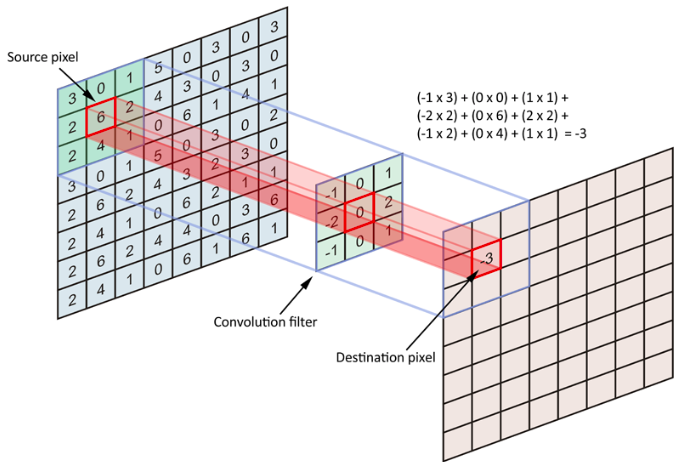
\includegraphics[width=\textwidth]{images/2d-Conv.png}
    \caption{Example of a single 3x3 convolution operation. The source image is convolved with a 3x3 kernel. The kernel's weights are determined using backpropagation.}
    \label{fig:code:2DConv}
\end{figure}

\label{sec:code:inceptnet}

The inceptnet architecture \cite{https://doi.org/10.48550/arxiv.1409.4842} has been demonstrated by D. Böckenhoff et al. \cite{Böckenhoff_2019} to be effective on a simplified version of this problem and by M. Blatzheim et al. \cite{Blatzheim_2019} to be effective on data from the same divertor configuration. In initial tests it was very promising for this application and met an important boundary conditions, mainly the network fit into the available video memory on the system used to train the network. Inceptnet uses a series of sub-networks, known as inception modules (see fig. \ref{fig:code:inceptmodule}). Each inception module is made up of 3 convolutional paths (1x1, 3x3, and 5x5) and a pooling path. To assure the outputs from each path have the same resolution, padding is added to the 3x3 and 5x5 convolutions. The number of each convolutional filter can be adjusted at each step and the outputs are concatenated together. The idea behind having multiple convolution sizes is that some features of the input might be lost if only size of kernel is applied.

\begin{figure}[htb]
    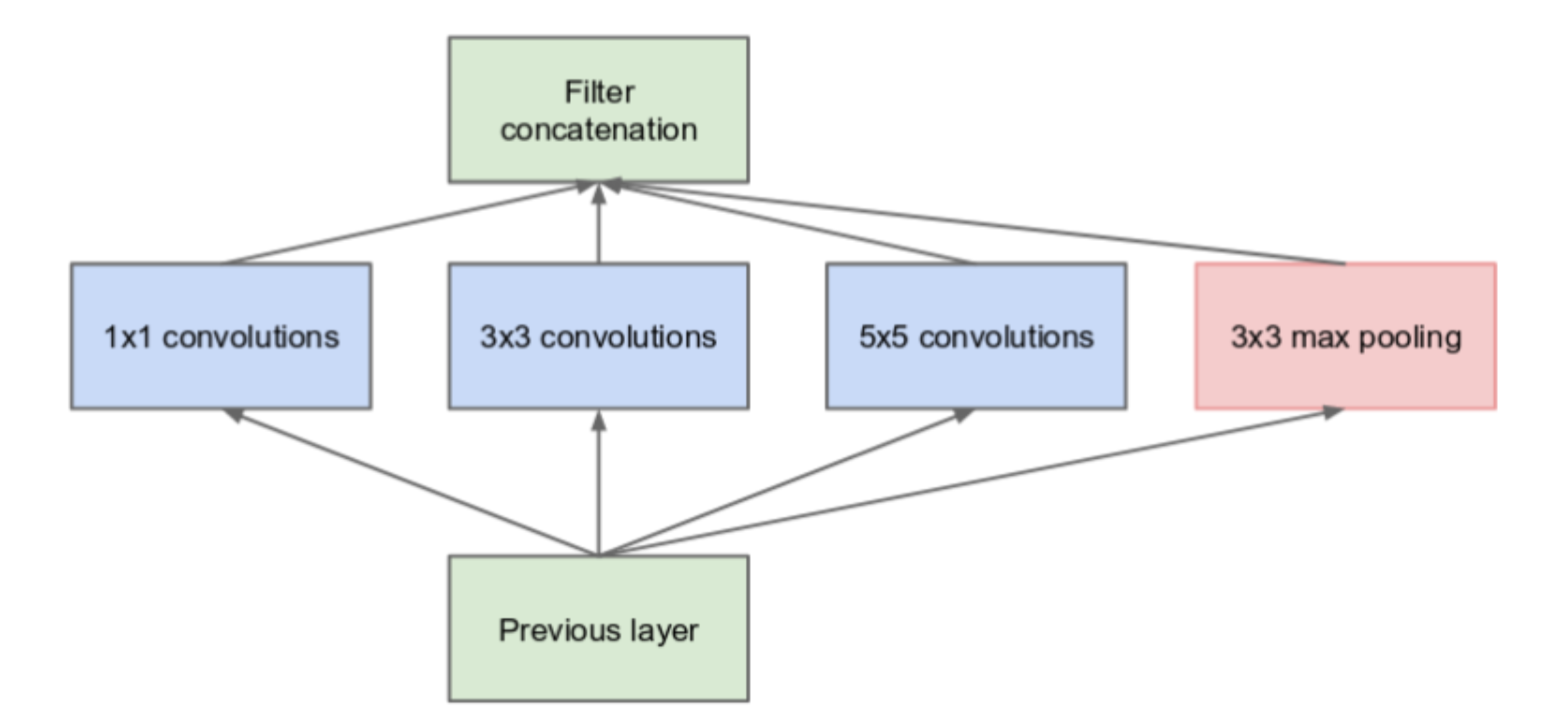
\includegraphics[width=\textwidth]{images/incept-simple.png}
    \caption{A diagram of the inception module. The inputs from the prior layer are fed into 4 paths, applying 1x1, 3x3, 5x5, convolutions with the final layer being 3x3 max pooling. The outputs of each layer are concatenated and passed to the next incept module. The number of 1x1, 3x3, and 5x5 convolutions per incept module can be adjusted.}
    \label{fig:code:inceptmodule}
\end{figure}

Each of the paths in the four branches of the inception module play a different role. The 1x1 filter doesn't take into account any patterns in the inputs height and width, but it does work across channels (depth) of the image. This acts to reduce the dimension of the input while connecting the values from the other channels of the input. The 1x1 convolution can also be used to reduce the number of channels as the output of the filter will be 1x1x$n$, where $n$ is the number of 1x1 filters being applied \cite{https://doi.org/10.48550/arxiv.1312.4400}. This is why each branch has a 1x1 convolution. The 1x1 convolutions marked in yellow in fig. \ref{fig:code:inceptmodule} are designed to reduce the number of channels input to the higher computational cost which dramatically reduces the number of weights needed for a module.

The 3x3 and 5x5 convolutions look at spacial patterns across the width, height, and depth of the input. In this way they are actually a 3-dimensional convolution, but most convolutions are referred to by their 2-dimensional cross-section. These two filters are typical optimized for finding features of the input at different scales. Prior to this multi-branch approach, machine learning scientists would hand select the ordering of the various convolution sizes to be applied in succession. By providing multiple paths and allowing the training process to determine which branches are necessary for a given step takes the human bias out of the training process in this regard.

There are several other structures that appear in the inception module. One being a 3x3 max pooling layer, which is like a 3x3 convolution, but instead of taking the element-wise product with the filter, it returns the max pixel value over the region of the feature map that overlaps with the filter. Pooling layers are a method of downsampling the input while attempting to preserve the most relevant pixels and are a staple of most deep convolutional networks. The concatenation layer just concatenates the outputs from the various branches together. Each branch has padding so that the height and width channels are aligned to make concatenation simple.

Lastly, there are batch normalization layers after every operation on each brach of the inception module. Batch normalization is powerful tool in any deep learning model. It has been shown that batch normalization solves the issue of internal covariate shift, where layers in the network shift the input distribution to the next layer \cite{https://doi.org/10.48550/arxiv.1502.03167}. Since the inputs of any layer in the network are affected by the weights of every prior layer, small changes in the distribution get amplified as they propagate throughout the network. To address this during training batches of data are normalized, transforming the neurons output using the first and second statistical moments (mean and standard deviation) across the batch. Two additional trainable parameters, $\gamma$ and $\beta$ are applied after normalization to specify the output distribution, so each layer can achieve a unique output distribution based on the optimal one for the next operation or layer.

Incept modules also have two major advantages over classic deep convolutional networks, they require far fewer parameters, which reduced the overall memory footprint of the model and far fewer floating point operations than prior convolutional modules. For example, using a 5x5 convolution to produce the same number of output channels as a incept module requires over 7 times the number of model parameters and floating point operations compared to the incept module. However, despite having significantly fewer model parameters, when the inceptnet was release, it was the state of the art architecture. Inceptnet outperformed models with the higher parameter count 5x5 and 3x3 modules.

The inception modules are stacked repeatedly (see fig. \ref{diagram:inceptnet}), varying the number of filters in each brach of the incept modules in each layer of modules. Eight total inception modules were used in the network with an input and output network, which can be seen as the repeating structures in the figure.

The input network is a 2D convolution used to scale up the number of channels. Since the graph representation of the network is too fine to be clear in this format, the figure \ref{diagram:inceptnet-in} takes a closer look at the input network and the first incept module. The output network flattens the output and passes it through a 128 neuron fully connected layer before reducing it to the output dimension of the network. While this was a reduction in the original scale of the Inceptnet design because the input images are higher resolution there are far more weights per step. For example, with an image resolution of 80\% of the original image size (260x1040 pixels) and a batch si ze of 10, the amount of ram needed to store the weights for the forward and back propagation step alone is 21.4 GB, which exceeds the video memory of all but the highest end consumer graphics cards. Since one of the questions being addressed by this thesis will be the impact of scaling the input image resolution on the accuracy, it is important to design a model that runs with the hardware available.

\begin{figure}
    \centering
    \includegraphics[width=\paperwidth, height=\textheight, keepaspectratio]{images/inceptnet.png}
    \caption{A diagram of the entire inception network as used in this paper.}
    \label{diagram:inceptnet}
\end{figure}

\begin{figure}
    \centering
    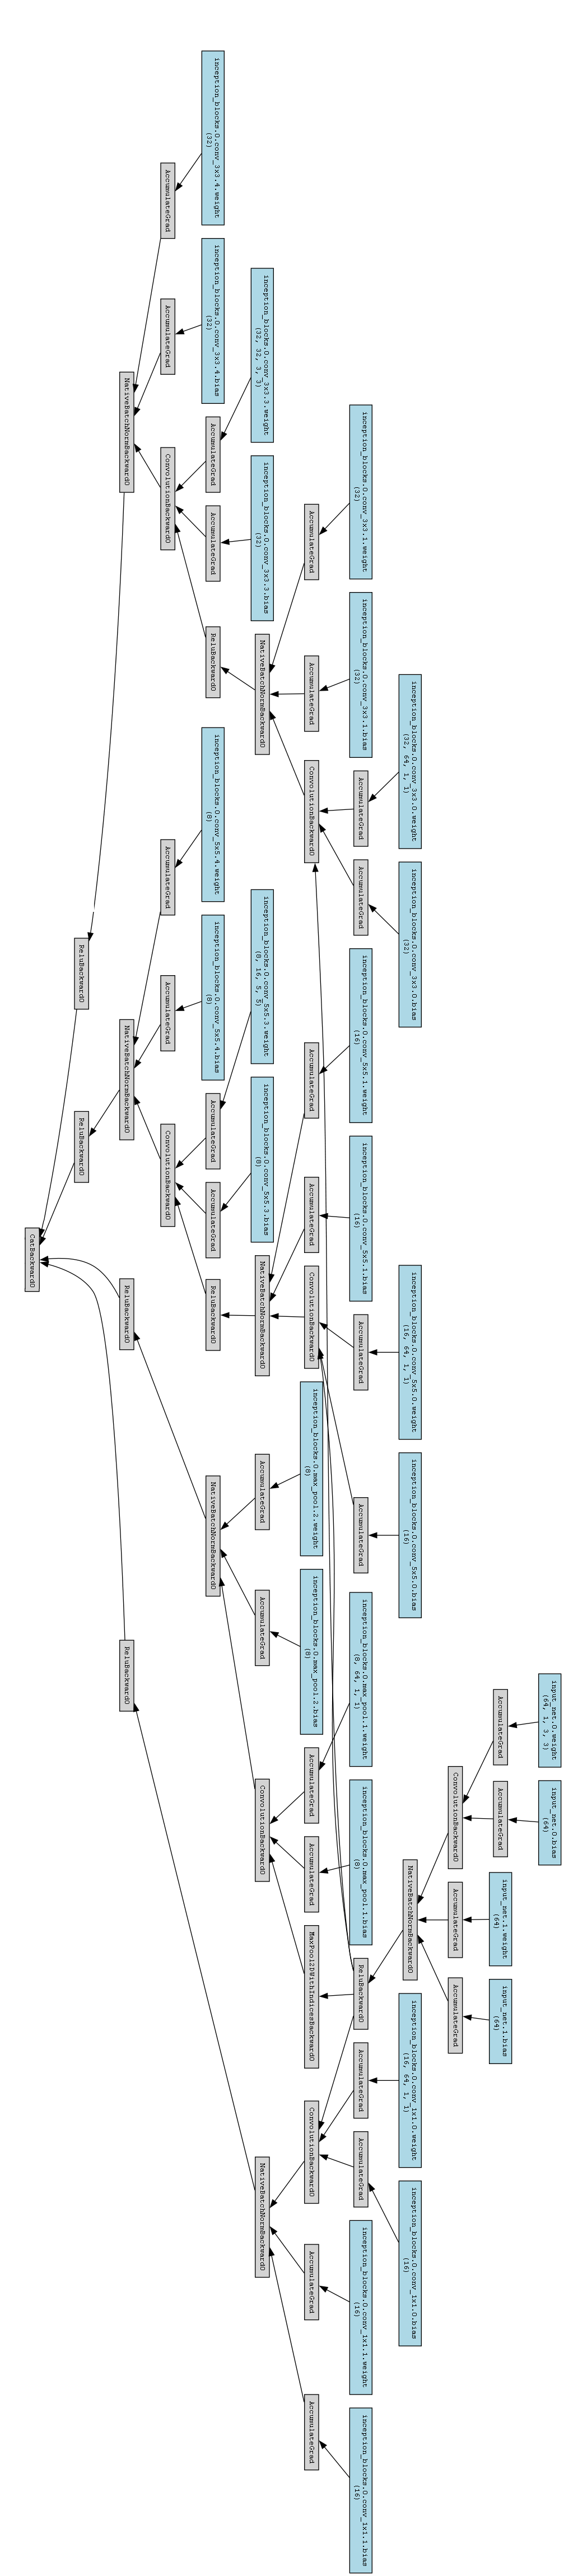
\includegraphics[width=\paperwidth, height=\textheight, keepaspectratio]{images/graph-input.png}
    \caption{A subsection of \ref{diagram:inceptnet} diagram looking at the input network and the first inception module.}
    \label{diagram:inceptnet-in}
\end{figure}

\label{sec:code:hyperparameters}

Once the broad architecture was selected the next step is to tune the model. Tuning the model helps model level parameters, like the number of filters at a given module, to be optimized for the use case. Tuning was done systematically with Optuna \cite{optuna} and results were recorded and compared using Tensorboard \cite{tensorboard} and MLFlow \cite{mlflow}.

The labels of the data set are the expected values the network will output given a specific input. $\iota$, the rotational transform or the ratio of poloidal transits per toroidal turn of any field line on a flux surface, is the label used for training. Initially, the labels for the data set were not available since simulations were necessary to produce them and that process is computationally expensive. Instead, simplified versions of the labels which just took into account the sum of $I_A$ and $I_B$, which provides a good first order approximation. Naturally, this will neglect the plasmas induced changes to the magnetic field. Simulations using VMEC allowed for a more accurate approximation for $\iota$. However, it is prohibitively computationally intensive to run 22,000+ simulations using extender, a simulation tool necessary for extending the results from VMEC to regions outside of the plasma and the field line tracer, a tool used for tracking field lines from the area outside of the plasma to the internal PFCs. The compromise is to use a value of $\iota$ at the edge of the plasma, as the VMEC simulations can be made much faster alone.

\label{sec:code:philosophy}
The design philosophy of this project was important. The code was designed to be a complete package, to be easily used by fellow colleges, and to work with the state of the art tools available in the machine learning space. PyTorch \cite{pytorch} was used at the primary framework, as many of members of the NEISS group used this as well. The PyTorch Lightning \cite{pytorch_lightning} package provided a powerful way to design an object-oriented machine learning package. For lower-level operations, like managing and recording the network configuration files, hyperparmeter searches, as well as structuring and analyzing results, the package Hydra \cite{hydra}, developed by Facebook, was used. Git \cite{git} was used for the version control system and DVC \cite{dvc} for data version control. This project was profiled and optimized with help from the PyTorch Lightning profiler. Code comments and documentation have been developed to help with quick adoption of the code for future use.

Since future changes to the divertor surface will result in drastically different inputs to the network, the code was designed to automatically scale with the inputs. The design philosophy was focused on making a project that could be quickly and easily taken over by a future student and be powerful and flexible enough to work with expected changes in the future. Reguardless of whether or not the code will never used again it is still a valuable lesson in Python software development and MLops. All of the code is available on GitHub at the following link:

\url{https://github.com/natephysics/hfcnn}